\documentclass[a4paper]{article}

\usepackage[utf8]{inputenc}
\usepackage[T1]{fontenc}
\usepackage{graphicx}
\usepackage{geometry}
\usepackage{setspace}
\usepackage{titling}
\usepackage{float}


\geometry{margin=2.5cm}
\setstretch{1.15}

\renewcommand{\contentsname}{Índice}
\renewcommand{\figurename}{Figura}
\renewcommand{\tablename}{Tabla}
\renewcommand{\refname}{Referencias}

\begin{document}

\begin{titlepage}
    \centering

    \vspace*{1.5cm}

    {\Huge \bfseries Mantenimiento basado en la condición de las plantas propulsoras navales.\par}

    \vspace{0.35cm}

    {\Large
    Analítica de Datos para la Industria
    \par}

    \vspace{0.75cm}

    {\large
    \textbf{Autores}\\[0.25cm]

    Markel Adánez$^{1}$ \qquad
    Unai López$^{1}$ \qquad
    Ander Arrondo$^{1}$
    \par}

    \vspace{0.75cm}

    {\large
    \textbf{Universidad de Deusto}$^{1}$\\[0.15cm]
    Facultad de Ingeniería
    \par}
    \vspace{0.25cm}
    {\small \today\par}

    \vspace{0.5cm}

    
\includegraphics[width=0.25\textwidth]{media/deusto.png}

    \vspace{0.5cm}

    \begin{minipage}{0.9\textwidth}
        {\centering
          \textbf{\large Resumen}\par
        }

        \vspace{0.3cm}

        \small
        Lorem ipsum dolor sit amet, consectetur adipiscing elit, sed do eiusmod tempor incididunt ut labore et dolore magna aliqua. Ut enim ad minim veniam, quis nostrud exercitation ullamco laboris nisi ut aliquip ex ea commodo consequat. Duis aute irure dolor in reprehenderit in voluptate velit esse cillum dolore eu fugiat nulla pariatur. Excepteur sint occaecat cupidatat non proident, sunt in culpa qui officia deserunt mollit anim id est laborum.
    \end{minipage}
    
    \begin{figure}[H]
      \centering
      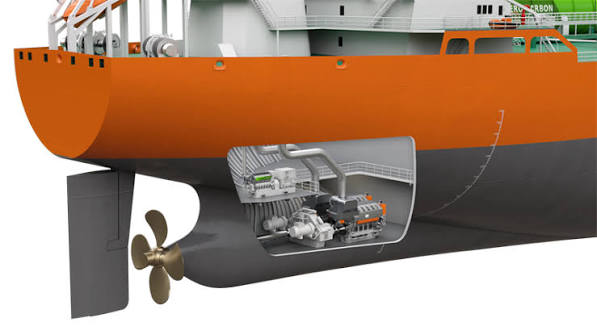
\includegraphics[width=0.8\textwidth]{media/naval_propulsion_plant.jpg}
      \caption{Ejemplo de la estructura de un propulsor naval.~\cite{wartsila_rina_novel_propulsion_arrangement_2021}}
      \label{fig:estructura-propulsor}
    \end{figure}

\end{titlepage}

\tableofcontents

\newpage


\section{Introducción}
  % Introducción de la temática a tratar.
  Según la \textit{Organización Mundial del Comercio} (OMC) el transporte marítimo representa más del 80\% del volumen del comercio mundial. Esto es, una gran mayoría de los bienes comerciales son suministrados a través del mar, de tal manera que este método de transporte constituye la columna vertebral de las cadenas de suministro mundiales.~\cite{condition_based_maintenance_of_naval_propulsion_plants_316}
  
  Los cargueros navales son propulsados por maquinarias (véase la Figura~\ref{fig:estructura-propulsor}) que han de resistir grandes fuerzas y vibraciones por parte del oleaje durante largos viajes y empujar masas de tamaño considerable a través de las aguas. En consecuencia, es imperativo asegurarse de la durabilidad y el correcto funcionamiento de los propulsores. En caso contrario, muchos barcos transportadores quedarían a la deriva interrumpiendo el comercio global y generando escasez en muchos sectores críticos de la economía.

\section{Sobre el conjunto de datos}
  % Origen del conjunto de datos (¿de dónde se ha obtenido?), el tipo de datos que contiene (¿cómo
  % están estructurados? ¿Qué tamaño tiene el dataset?), así como el contexto (¿qué representa?, ¿en
  % qué circunstancias o escenarios industriales se recopilaron estos datos?)

\section{Sobre el dominio}
  % Contextualización del conjunto de datos (¿qué eventos o tendencias industriales llevaron a su
  % creación o necesidad?) y terminología (¿qué conceptos se deben comprender? - definición y
  % descripción de los términos clave relacionados con el conjunto de datos).

\section{Definición del problema}
  % Enfoque del estudio de los datos (¿qué problema específico se propone resolver o responder con este
  % conjunto de datos?), justificación (¿por qué es relevante o crítico abordar este problema en el
  % contexto industrial actual?)

\section{Objetivos e hipótesis}
  % Planteamiento de que se pretende abordar (¿qué se espera descubrir o inferir de este conjunto de
  % datos?), plantear posibles causas para la problemática a abordar en función de lo que se esté
  % estudiando, objetivos del estudio. 

\section{Metodología propuesta}
  % Aunque no se realizará un análisis práctico en esta etapa, describir las técnicas o enfoques analíticos
  % que se considerarían para abordar el problema. Es decir, pasos iniciales para su estudio (ingesta,
  % verificación datos, detección valores anómalos …), describir las pautas tentativas para el análisis
  % exploratorio (balance del dataset, clases/outputs esperadas, variables de interés, estudio
  % distribuciones…), posibles modelos estrategias de análisis en función e los datos de los que se dispone
  % (no tanto las técnicas, si no su planteamiento desde el punto de vista de input/output)... En definitiva,
  % el proceso que se espera seguir en el análisis de los datos. 

\bibliographystyle{plain}
\bibliography{references}

\end{document}
